
%(BEGIN_QUESTION)
% Copyright 2011, Tony R. Kuphaldt, released under the Creative Commons Attribution License (v 1.0)
% This means you may do almost anything with this work of mine, so long as you give me proper credit

Suppose the following control system is functioning as it is designed to, under regular operating conditions (i.e. 25 feet of water measured in the well, with a normal amount of water flow to the customers).  The pump's discharge pressure is holding perfectly at its setpoint value of 95 PSI:

$$\includegraphics[width=15.5cm]{i02973x01.eps}$$

\noindent
Choose the best answer describing the immediate effect on this process if the level transmitter suddenly fails with a {\it high} signal:

\begin{itemize}
\item{} The pump's discharge pressure will immediately begin to fall below setpoint
\vskip 10pt
\item{} The system will continue to operate normally, maintaining 95 PSI to the customers
\vskip 10pt
\item{} The water level in the well will begin to slowly fall as more water is drawn out
\vskip 10pt
\item{} The pump's discharge pressure will immediately begin to rise above setpoint
\end{itemize}

\underbar{file i02973}
%(END_QUESTION)





%(BEGIN_ANSWER)

The system will continue to operate normally, maintaining 95 PSI to the customers

%(END_ANSWER)





%(BEGIN_NOTES)

{\bf This question is intended for exams only and not worksheets!}.

%(END_NOTES)


